% Created by tikzDevice version 0.8.1 on 2015-06-28 01:47:35
% !TEX encoding = UTF-8 Unicode
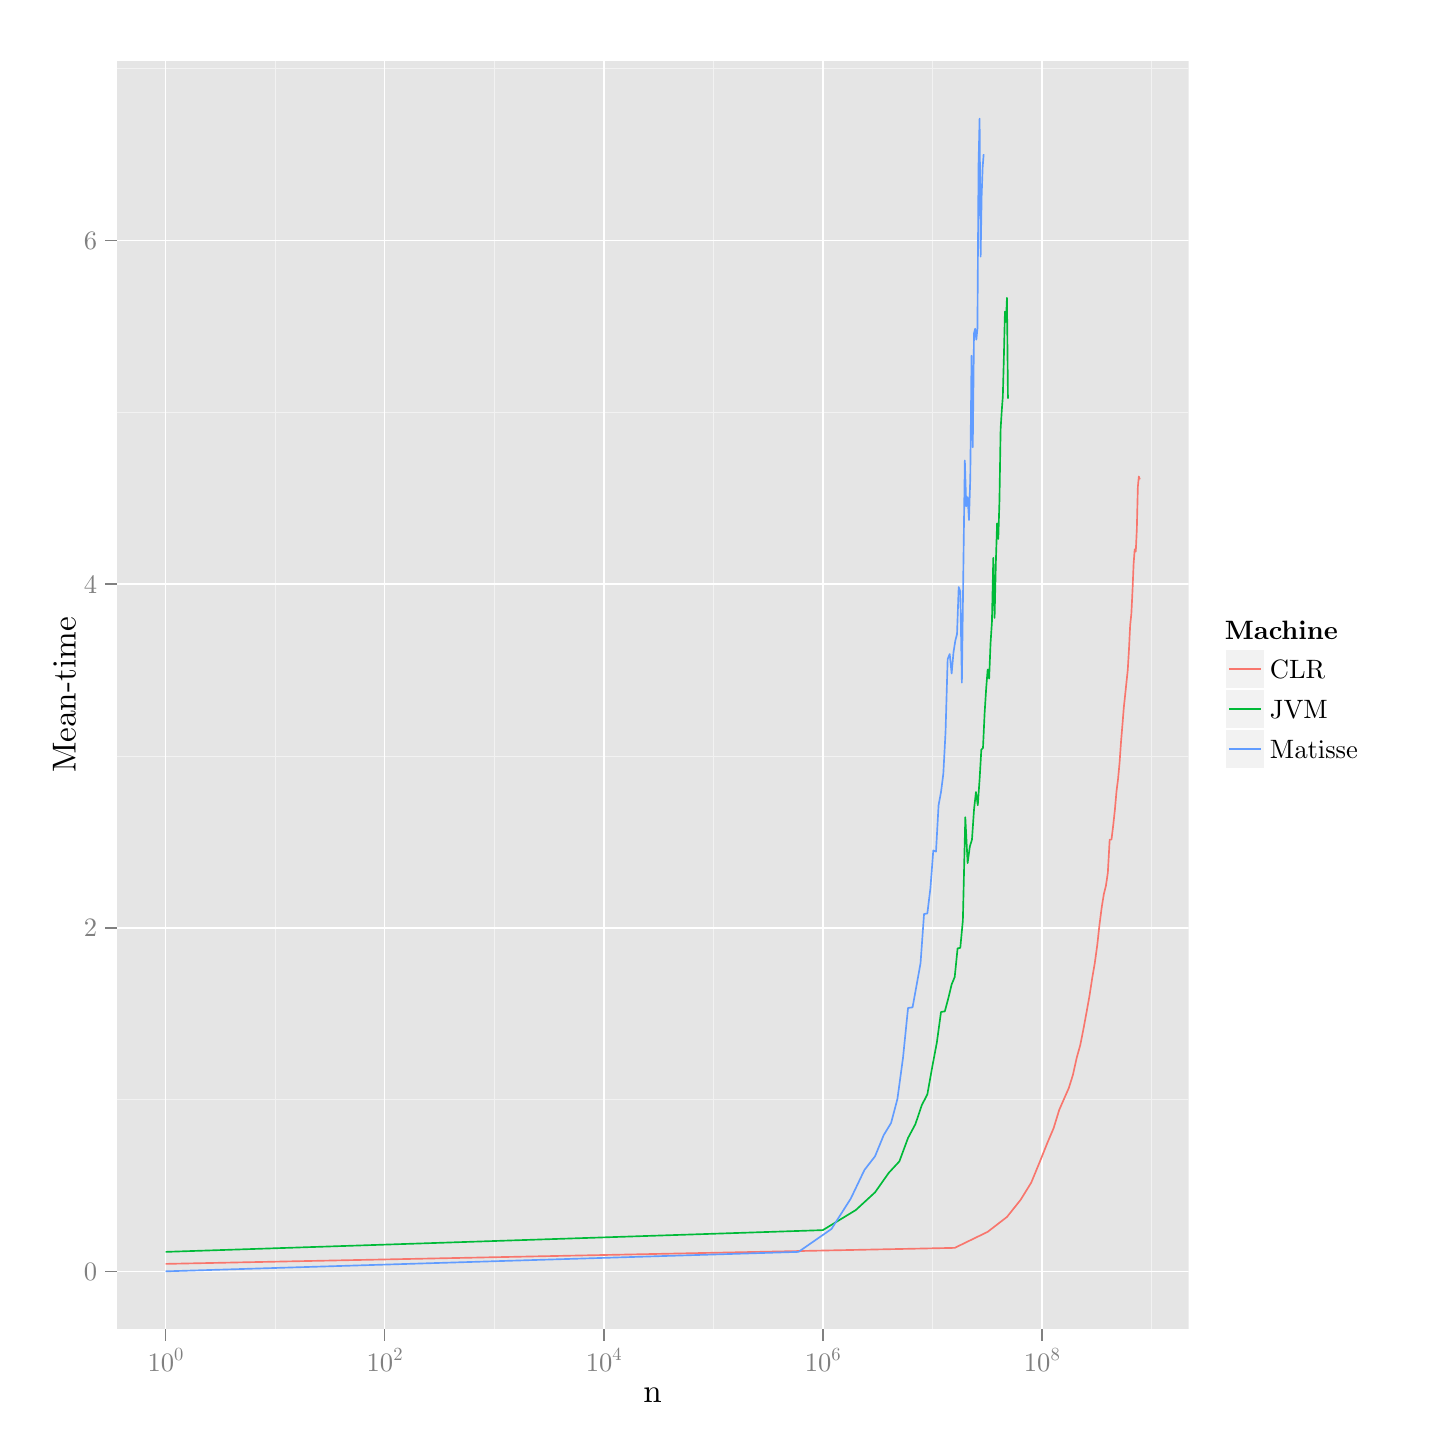
\begin{tikzpicture}[x=1pt,y=1pt]
\definecolor{fillColor}{RGB}{255,255,255}
\path[use as bounding box,fill=fillColor,fill opacity=0.00] (0,0) rectangle (505.89,505.89);
\begin{scope}
\path[clip] (  0.00,  0.00) rectangle (505.89,505.89);
\definecolor{drawColor}{RGB}{255,255,255}
\definecolor{fillColor}{RGB}{255,255,255}

\path[draw=drawColor,line width= 0.6pt,line join=round,line cap=round,fill=fillColor] (  0.00,  0.00) rectangle (505.89,505.89);
\end{scope}
\begin{scope}
\path[clip] ( 32.22, 35.66) rectangle (419.48,493.85);
\definecolor{fillColor}{gray}{0.90}

\path[fill=fillColor] ( 32.22, 35.66) rectangle (419.48,493.85);
\definecolor{drawColor}{gray}{0.95}

\path[draw=drawColor,line width= 0.3pt,line join=round] ( 32.22,118.56) --
	(419.48,118.56);

\path[draw=drawColor,line width= 0.3pt,line join=round] ( 32.22,242.72) --
	(419.48,242.72);

\path[draw=drawColor,line width= 0.3pt,line join=round] ( 32.22,366.87) --
	(419.48,366.87);

\path[draw=drawColor,line width= 0.3pt,line join=round] ( 32.22,491.02) --
	(419.48,491.02);

\path[draw=drawColor,line width= 0.3pt,line join=round] ( 89.41, 35.66) --
	( 89.41,493.85);

\path[draw=drawColor,line width= 0.3pt,line join=round] (168.57, 35.66) --
	(168.57,493.85);

\path[draw=drawColor,line width= 0.3pt,line join=round] (247.73, 35.66) --
	(247.73,493.85);

\path[draw=drawColor,line width= 0.3pt,line join=round] (326.90, 35.66) --
	(326.90,493.85);

\path[draw=drawColor,line width= 0.3pt,line join=round] (406.06, 35.66) --
	(406.06,493.85);
\definecolor{drawColor}{RGB}{255,255,255}

\path[draw=drawColor,line width= 0.6pt,line join=round] ( 32.22, 56.49) --
	(419.48, 56.49);

\path[draw=drawColor,line width= 0.6pt,line join=round] ( 32.22,180.64) --
	(419.48,180.64);

\path[draw=drawColor,line width= 0.6pt,line join=round] ( 32.22,304.79) --
	(419.48,304.79);

\path[draw=drawColor,line width= 0.6pt,line join=round] ( 32.22,428.94) --
	(419.48,428.94);

\path[draw=drawColor,line width= 0.6pt,line join=round] ( 49.82, 35.66) --
	( 49.82,493.85);

\path[draw=drawColor,line width= 0.6pt,line join=round] (128.99, 35.66) --
	(128.99,493.85);

\path[draw=drawColor,line width= 0.6pt,line join=round] (208.15, 35.66) --
	(208.15,493.85);

\path[draw=drawColor,line width= 0.6pt,line join=round] (287.32, 35.66) --
	(287.32,493.85);

\path[draw=drawColor,line width= 0.6pt,line join=round] (366.48, 35.66) --
	(366.48,493.85);
\definecolor{drawColor}{RGB}{248,118,109}

\path[draw=drawColor,line width= 0.6pt,line join=round] ( 49.82, 59.18) --
	(334.98, 64.97) --
	(346.89, 70.76) --
	(353.86, 76.14) --
	(358.81, 82.35) --
	(362.64, 88.56) --
	(365.78, 96.21) --
	(368.43,102.84) --
	(370.72,108.22) --
	(372.75,114.84) --
	(374.56,118.98) --
	(376.20,122.70) --
	(377.69,127.46) --
	(379.07,133.67) --
	(380.34,138.22) --
	(381.53,144.22) --
	(382.64,150.22) --
	(383.68,156.02) --
	(384.66,162.43) --
	(385.59,167.81) --
	(386.47,174.22) --
	(387.31,181.88) --
	(388.11,188.09) --
	(388.88,192.85) --
	(389.61,195.74) --
	(390.31,200.50) --
	(390.98,212.50) --
	(391.63,212.50) --
	(392.26,217.68) --
	(392.86,223.26) --
	(393.44,229.89) --
	(394.01,234.44) --
	(394.55,240.23) --
	(395.08,247.89) --
	(395.60,254.10) --
	(396.09,260.30) --
	(396.58,264.86) --
	(397.05,269.41) --
	(397.51,273.75) --
	(397.95,281.20) --
	(398.39,290.10) --
	(398.81,294.03) --
	(399.23,302.52) --
	(399.63,312.24) --
	(400.03,317.41) --
	(400.41,316.59) --
	(400.79,324.66) --
	(401.16,339.97) --
	(401.52,343.69) --
	(401.88,342.66);
\definecolor{drawColor}{RGB}{0,186,56}

\path[draw=drawColor,line width= 0.6pt,line join=round] ( 49.82, 63.52) --
	(287.32, 71.38) --
	(299.23, 78.63) --
	(306.20, 85.04) --
	(311.15, 92.08) --
	(314.98, 96.21) --
	(318.12,104.70) --
	(320.77,109.66) --
	(323.06,116.49) --
	(325.09,120.42) --
	(326.90,130.56) --
	(328.54,139.25) --
	(330.03,150.22) --
	(331.41,150.43) --
	(332.68,155.19) --
	(333.87,160.15) --
	(334.98,162.84) --
	(336.02,173.19) --
	(337.00,173.40) --
	(337.93,183.33) --
	(338.81,220.57) --
	(339.65,204.02) --
	(340.45,210.02) --
	(341.22,212.50) --
	(341.95,223.26) --
	(342.65,229.68) --
	(343.32,224.92) --
	(343.97,234.23) --
	(344.60,244.99) --
	(345.20,245.61) --
	(345.78,258.03) --
	(346.35,267.13) --
	(346.89,273.96) --
	(347.42,270.65) --
	(347.93,283.48) --
	(348.43,291.13) --
	(348.92,314.31) --
	(349.39,292.58) --
	(349.85,312.65) --
	(350.29,326.73) --
	(350.73,321.14) --
	(351.15,335.00) --
	(351.57,360.87) --
	(351.97,367.28) --
	(352.37,372.66) --
	(352.75,386.94) --
	(353.13,403.29) --
	(353.50,399.56) --
	(353.86,408.25) --
	(354.22,371.83);
\definecolor{drawColor}{RGB}{97,156,255}

\path[draw=drawColor,line width= 0.6pt,line join=round] ( 49.82, 56.49) --
	(278.53, 63.52) --
	(290.45, 71.80) --
	(297.42, 82.77) --
	(302.36, 93.11) --
	(306.20, 98.08) --
	(309.33,105.73) --
	(311.98,110.08) --
	(314.28,118.77) --
	(316.30,133.67) --
	(318.12,151.67) --
	(319.75,151.88) --
	(321.25,160.15) --
	(322.63,167.81) --
	(323.90,185.60) --
	(325.09,185.81) --
	(326.20,194.92) --
	(327.24,208.57) --
	(328.22,208.16) --
	(329.15,224.92) --
	(330.03,229.68) --
	(330.87,236.30) --
	(331.67,251.41) --
	(332.43,277.68) --
	(333.17,279.55) --
	(333.87,272.51) --
	(334.54,280.17) --
	(335.19,284.31) --
	(335.82,286.79) --
	(336.42,303.76) --
	(337.00,302.10) --
	(337.57,269.20) --
	(338.11,310.79) --
	(338.64,349.49) --
	(339.15,332.93) --
	(339.65,336.24) --
	(340.14,327.97) --
	(340.61,343.28) --
	(341.06,387.35) --
	(341.51,354.25) --
	(341.95,395.42) --
	(342.37,397.08) --
	(342.79,393.15) --
	(343.19,397.08) --
	(343.59,456.46) --
	(343.97,473.02) --
	(344.35,423.15) --
	(344.72,445.29) --
	(345.08,455.43) --
	(345.44,460.19);
\end{scope}
\begin{scope}
\path[clip] (  0.00,  0.00) rectangle (505.89,505.89);
\definecolor{drawColor}{gray}{0.50}

\node[text=drawColor,anchor=base east,inner sep=0pt, outer sep=0pt, scale=  0.96] at ( 25.11, 53.18) {0};

\node[text=drawColor,anchor=base east,inner sep=0pt, outer sep=0pt, scale=  0.96] at ( 25.11,177.33) {2};

\node[text=drawColor,anchor=base east,inner sep=0pt, outer sep=0pt, scale=  0.96] at ( 25.11,301.49) {4};

\node[text=drawColor,anchor=base east,inner sep=0pt, outer sep=0pt, scale=  0.96] at ( 25.11,425.64) {6};
\end{scope}
\begin{scope}
\path[clip] (  0.00,  0.00) rectangle (505.89,505.89);
\definecolor{drawColor}{gray}{0.50}

\path[draw=drawColor,line width= 0.6pt,line join=round] ( 27.95, 56.49) --
	( 32.22, 56.49);

\path[draw=drawColor,line width= 0.6pt,line join=round] ( 27.95,180.64) --
	( 32.22,180.64);

\path[draw=drawColor,line width= 0.6pt,line join=round] ( 27.95,304.79) --
	( 32.22,304.79);

\path[draw=drawColor,line width= 0.6pt,line join=round] ( 27.95,428.94) --
	( 32.22,428.94);
\end{scope}
\begin{scope}
\path[clip] (  0.00,  0.00) rectangle (505.89,505.89);
\definecolor{drawColor}{gray}{0.50}

\path[draw=drawColor,line width= 0.6pt,line join=round] ( 49.82, 31.39) --
	( 49.82, 35.66);

\path[draw=drawColor,line width= 0.6pt,line join=round] (128.99, 31.39) --
	(128.99, 35.66);

\path[draw=drawColor,line width= 0.6pt,line join=round] (208.15, 31.39) --
	(208.15, 35.66);

\path[draw=drawColor,line width= 0.6pt,line join=round] (287.32, 31.39) --
	(287.32, 35.66);

\path[draw=drawColor,line width= 0.6pt,line join=round] (366.48, 31.39) --
	(366.48, 35.66);
\end{scope}
\begin{scope}
\path[clip] (  0.00,  0.00) rectangle (505.89,505.89);
\definecolor{drawColor}{gray}{0.50}

\node[text=drawColor,anchor=base west,inner sep=0pt, outer sep=0pt, scale=  0.96] at ( 43.35, 20.31) {10};

\node[text=drawColor,anchor=base west,inner sep=0pt, outer sep=0pt, scale=  0.67] at ( 52.94, 24.24) {0};

\node[text=drawColor,anchor=base west,inner sep=0pt, outer sep=0pt, scale=  0.96] at (122.51, 20.31) {10};

\node[text=drawColor,anchor=base west,inner sep=0pt, outer sep=0pt, scale=  0.67] at (132.11, 24.24) {2};

\node[text=drawColor,anchor=base west,inner sep=0pt, outer sep=0pt, scale=  0.96] at (201.67, 20.31) {10};

\node[text=drawColor,anchor=base west,inner sep=0pt, outer sep=0pt, scale=  0.67] at (211.27, 24.24) {4};

\node[text=drawColor,anchor=base west,inner sep=0pt, outer sep=0pt, scale=  0.96] at (280.84, 20.31) {10};

\node[text=drawColor,anchor=base west,inner sep=0pt, outer sep=0pt, scale=  0.67] at (290.43, 24.24) {6};

\node[text=drawColor,anchor=base west,inner sep=0pt, outer sep=0pt, scale=  0.96] at (360.00, 20.31) {10};

\node[text=drawColor,anchor=base west,inner sep=0pt, outer sep=0pt, scale=  0.67] at (369.60, 24.24) {8};
\end{scope}
\begin{scope}
\path[clip] (  0.00,  0.00) rectangle (505.89,505.89);
\definecolor{drawColor}{RGB}{0,0,0}

\node[text=drawColor,anchor=base,inner sep=0pt, outer sep=0pt, scale=  1.20] at (225.85,  9.03) {n};
\end{scope}
\begin{scope}
\path[clip] (  0.00,  0.00) rectangle (505.89,505.89);
\definecolor{drawColor}{RGB}{0,0,0}

\node[text=drawColor,rotate= 90.00,anchor=base,inner sep=0pt, outer sep=0pt, scale=  1.20] at ( 17.30,264.75) {Mean-time};
\end{scope}
\begin{scope}
\path[clip] (  0.00,  0.00) rectangle (505.89,505.89);
\definecolor{fillColor}{RGB}{255,255,255}

\path[fill=fillColor] (428.35,233.68) rectangle (484.98,295.82);
\end{scope}
\begin{scope}
\path[clip] (  0.00,  0.00) rectangle (505.89,505.89);
\definecolor{drawColor}{RGB}{0,0,0}

\node[text=drawColor,anchor=base west,inner sep=0pt, outer sep=0pt, scale=  0.96] at (432.62,284.93) {\bfseries Machine};
\end{scope}
\begin{scope}
\path[clip] (  0.00,  0.00) rectangle (505.89,505.89);
\definecolor{drawColor}{RGB}{255,255,255}
\definecolor{fillColor}{gray}{0.95}

\path[draw=drawColor,line width= 0.6pt,line join=round,line cap=round,fill=fillColor] (432.62,266.86) rectangle (447.07,281.31);
\end{scope}
\begin{scope}
\path[clip] (  0.00,  0.00) rectangle (505.89,505.89);
\definecolor{drawColor}{RGB}{248,118,109}

\path[draw=drawColor,line width= 0.6pt,line join=round] (434.06,274.09) -- (445.62,274.09);
\end{scope}
\begin{scope}
\path[clip] (  0.00,  0.00) rectangle (505.89,505.89);
\definecolor{drawColor}{RGB}{255,255,255}
\definecolor{fillColor}{gray}{0.95}

\path[draw=drawColor,line width= 0.6pt,line join=round,line cap=round,fill=fillColor] (432.62,252.41) rectangle (447.07,266.86);
\end{scope}
\begin{scope}
\path[clip] (  0.00,  0.00) rectangle (505.89,505.89);
\definecolor{drawColor}{RGB}{0,186,56}

\path[draw=drawColor,line width= 0.6pt,line join=round] (434.06,259.63) -- (445.62,259.63);
\end{scope}
\begin{scope}
\path[clip] (  0.00,  0.00) rectangle (505.89,505.89);
\definecolor{drawColor}{RGB}{255,255,255}
\definecolor{fillColor}{gray}{0.95}

\path[draw=drawColor,line width= 0.6pt,line join=round,line cap=round,fill=fillColor] (432.62,237.95) rectangle (447.07,252.41);
\end{scope}
\begin{scope}
\path[clip] (  0.00,  0.00) rectangle (505.89,505.89);
\definecolor{drawColor}{RGB}{97,156,255}

\path[draw=drawColor,line width= 0.6pt,line join=round] (434.06,245.18) -- (445.62,245.18);
\end{scope}
\begin{scope}
\path[clip] (  0.00,  0.00) rectangle (505.89,505.89);
\definecolor{drawColor}{RGB}{0,0,0}

\node[text=drawColor,anchor=base west,inner sep=0pt, outer sep=0pt, scale=  0.96] at (448.88,270.78) {CLR};
\end{scope}
\begin{scope}
\path[clip] (  0.00,  0.00) rectangle (505.89,505.89);
\definecolor{drawColor}{RGB}{0,0,0}

\node[text=drawColor,anchor=base west,inner sep=0pt, outer sep=0pt, scale=  0.96] at (448.88,256.33) {JVM};
\end{scope}
\begin{scope}
\path[clip] (  0.00,  0.00) rectangle (505.89,505.89);
\definecolor{drawColor}{RGB}{0,0,0}

\node[text=drawColor,anchor=base west,inner sep=0pt, outer sep=0pt, scale=  0.96] at (448.88,241.87) {Matisse};
\end{scope}
\end{tikzpicture}
